% !TeX root = ../solution.tex

\hypertarget{he22.16}{%
\chapter{[HE22.16] Rabbits With Hats}\label{he22.16}}

\begin{marginfigure}
	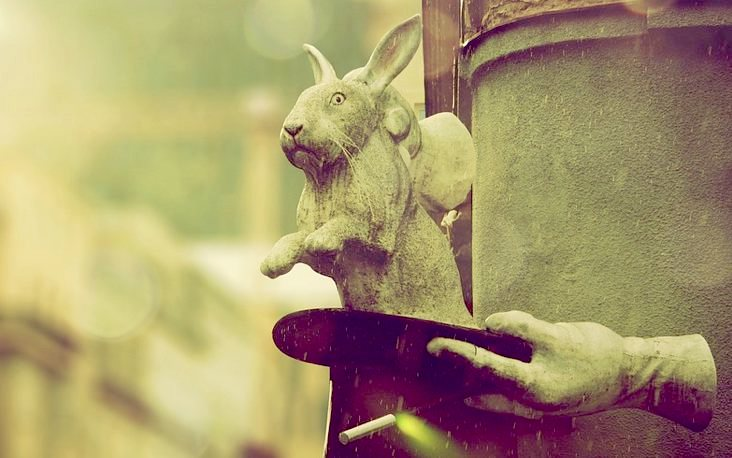
\includegraphics[width=49mm]{level5/challenge16.jpg}
\end{marginfigure}
\section{Intro}
I'm looking for a friend of mine who had to flee from his evil owner.

He must have found a shelter for wildlife, but didn't tell me where it is. He
just said he would go join rabbits with hats. What the heck do these three
words mean??

\noindent{\NotoEmoji 🚩} Flag
\begin{itemize}
\item \verb+he2022{nameoftheplace}+
\item \textbf{all lowercase, no spaces}
\item first letter is j, last one is y
\item e.g. \verb+he2022{junglezooaviary}+
\end{itemize}

\subsection{Hint}
\begin{itemize}
\item the number of words is important
\item search the nearby area
\end{itemize}    

\section{Solution}\label{hv22.16solution}
Do a goole search for \verb+three words rabbits with hats+ and it points you
to a map location and if you zoom out, there is the ``Jackrabbit Flat Wildlife
Sanctuary'' nearby.  So the flag is
\verb+he2022{he2022{jackrabbitflatwildlifesanctuary}+:


	









